%% LyX 2.3.6.1 created this file.  For more info, see http://www.lyx.org/.
%% Do not edit unless you really know what you are doing.
\documentclass[english]{article}
\usepackage[T1]{fontenc}
\usepackage[latin9]{inputenc}
\usepackage{geometry}
\geometry{verbose,tmargin=2.5cm,bmargin=2.5cm,lmargin=2.5cm,rmargin=2.5cm}
\usepackage{graphicx}

\makeatletter

%%%%%%%%%%%%%%%%%%%%%%%%%%%%%% LyX specific LaTeX commands.
%% Because html converters don't know tabularnewline
\providecommand{\tabularnewline}{\\}

\makeatother

\usepackage{babel}
\begin{document}
{[}SPLIT\_HERE{]}
\begin{enumerate}
\item \textbf{{[}PJC/PRELIM/9597/2017/P1/Q1{]} }

The text file \texttt{TEMPERATURE.txt} contains the mean daily temperature
from January 1982 to June 2017. Each line of record is in the format 
\noindent \begin{center}
\texttt{<year>-<month> <mean daily temperature> }
\par\end{center}

For examples, \texttt{1982-01 29.8} and \texttt{2017-06 31.6} 

\subsection*{Task 1.1 }

Write program code that will 
\begin{itemize}
\item read the data from the text file, 
\item calculate the average of all the available monthly temperatures by
year, by totalling up the temperatures for each month of that year
and divided by the number of months, 
\item output the average temperature for that year (from 1982 to 2017),
in 3 decimal places.
\item Use the following format: 
\noindent \begin{center}
\texttt{}%
\begin{tabular}{ccc}
\texttt{Year} &  & \texttt{Average temperature}\tabularnewline
\texttt{1982} &  & \texttt{31.442}\tabularnewline
\texttt{1983} &  & \texttt{31.750}\tabularnewline
\texttt{$\vdots$} &  & \texttt{$\vdots$}\tabularnewline
\texttt{$\vdots$} &  & \texttt{$\vdots$}\tabularnewline
\texttt{2017} &  & \texttt{31.217 }\tabularnewline
\end{tabular}\texttt{ }
\par\end{center}
\end{itemize}

\subsection*{Evidence 1: }

Program code for Task 1.1.\hfill{} {[}9{]}

\subsection*{Evidence 2: }

Screenshot of running program.\hfill{} {[}1{]}

\subsection*{Task 1.2 }

Sort by temperature and output the average temperature by year, in
ascending order of temperature. If temperatures are the same, then
display the later year before the earlier year. For example, if year
2017 and 1989 have the same temperature, then display 2017 before
1989. 

\subsection*{Evidence 3:}

Program code for Task 1.2. \hfill{}{[}7{]}

\subsection*{Evidence 4: }

Screenshot of running program. \hfill{}{[}1{]}

{[}SPLIT\_HERE{]}
\item \textbf{{[}PJC/PRELIM/9597/2017/P1/Q2{]} }

A circular queue is to be implemented with a fixed size array of n
elements, indexed from \texttt{0} to \texttt{(n \textendash{} 1)}.
\begin{center}
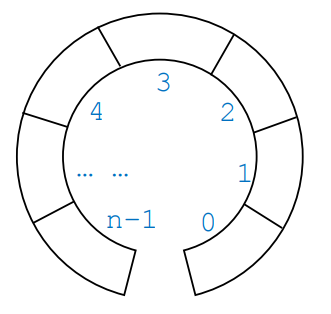
\includegraphics[width=0.2\paperwidth]{C:/Users/Admin/Desktop/Github/question_bank/LyX/static/img/9597-PJC-2017-P1-Q2-1}
\par\end{center}

\subsection*{Task 2.1 }

Following good programming practice, write program code for procedures 
\begin{itemize}
\item \texttt{setup\_queue} to set up circular queue which allows user to
input the value of \texttt{n}, 
\item \texttt{enqueue} to add an element to the queue,
\item \texttt{dequeue} to remove an element from the queue. 
\end{itemize}

\subsection*{Evidence 5: }

Program code for Task 2.1 for \texttt{setup\_queue}, \texttt{enqueue},
\texttt{dequeue}. \hfill{}{[}12{]}

\subsection*{Task 2.2 }

Write program code for a main procedure to display a menu with these
options: 
\noindent \begin{center}
\begin{tabular}{|l|}
\hline 
\texttt{1. Set up queue}\tabularnewline
\texttt{2. Add to queue}\tabularnewline
\texttt{3. Remove from queue}\tabularnewline
\texttt{4. Display queue }\tabularnewline
\texttt{5. Exit}\tabularnewline
\hline 
\end{tabular}
\par\end{center}

Write additional code to implement menu options 1, 2 and 3 using procedures
from Task 2.1. 

Also write code to implement 
\begin{itemize}
\item option 4 to display the contents of the queue and its pointers as
shown in diagram below, 
\item option 5 to exit program. 
\end{itemize}
The diagram shows the result of option 4 to display contents of queue
and pointers for \texttt{n=5} with 3 items \texttt{'fig'}, \texttt{'lemon'}
and \texttt{'cane'} in the queue:
\noindent \begin{center}
\begin{tabular}{l|l|l}
\multicolumn{1}{l}{} & \multicolumn{1}{l}{\texttt{Queue}} & \tabularnewline
 & \texttt{fig} & \texttt{<- Front pointer}\tabularnewline
 & \texttt{lemon} & \tabularnewline
 & \texttt{cane} & \texttt{<- Rear pointer}\tabularnewline
 &  & \tabularnewline
 &  & \tabularnewline
\multicolumn{1}{l}{} & \multicolumn{1}{l}{} & \tabularnewline
\multicolumn{1}{l}{} & \multicolumn{2}{l}{\texttt{Number in queue: 3}}\tabularnewline
\end{tabular}
\par\end{center}


\subsection*{Evidence 6:}

Program code for Task 2.2 for main procedure, display queue and exit
program. \hfill{}{[}8{]}

\subsection*{Task 2.3 }

Test run your program from using the following input: 
\noindent \begin{center}
\begin{tabular}{|l|}
\hline 
\texttt{Test run 1}\tabularnewline
\hline 
- \texttt{n = 8}\tabularnewline
- Add 5 words to queue in order:\tabularnewline
\texttt{'Mary', 'had', 'a', 'little', 'lamb'}\tabularnewline
- Display queue\tabularnewline
\hline 
\end{tabular}~~~~~~~~~~~%
\begin{tabular}{|l|}
\hline 
\texttt{Test run 2}\tabularnewline
\hline 
- \texttt{n = 3}\tabularnewline
- Add 4 words to queue in order:\tabularnewline
\texttt{'The', 'quick', 'brown', 'fox'}\tabularnewline
- Remove from queue\tabularnewline
- Display queue\tabularnewline
\hline 
\end{tabular}
\par\end{center}

\subsection*{Evidence 7 }

Screenshots of test runs 1 and 2. \hfill{}{[}2{]}

{[}SPLIT\_HERE{]}
\item \textbf{{[}PJC/PRELIM/9597/2017/P1/Q3{]} }

A linked list of nodes is used to store data for a college. The data
include name of student and exam mark. 

The linked list Abstract Data Type (ADT) has commands to create a
new linked list, add data items to the list and display the list. 

The program to implement this ADT will use the classes \texttt{Node}
and \texttt{LinkedList} as follows: 
\begin{center}
\begin{tabular}{|l|}
\hline 
\texttt{\hspace{0.25\columnwidth}Node}\tabularnewline
\hline 
\texttt{name : STRING}\tabularnewline
\texttt{mark : INTEGER}\tabularnewline
\texttt{nextPtr : INTEGER}\tabularnewline
\hline 
\texttt{constructor()}\tabularnewline
\texttt{setName(name : STRING)}\tabularnewline
\texttt{setMark(mark : INTEGER) }\tabularnewline
\texttt{setNextPtr(ptr : INTEGER)}\tabularnewline
\texttt{getName() : STRING}\tabularnewline
\texttt{getMark() : INTEGER}\tabularnewline
\texttt{getNextPtr() : INTEGER}\tabularnewline
\hline 
\end{tabular}~~~~~~%
\begin{tabular}{|l|}
\hline 
\texttt{\hspace{0.25\columnwidth}LinkedList}\tabularnewline
\hline 
\texttt{nodes : ARRAY OF Node}\tabularnewline
\texttt{head : INTEGER}\tabularnewline
\hline 
\texttt{constructor()}\tabularnewline
\texttt{addInOrder(name, mark)}\tabularnewline
\texttt{print() }\tabularnewline
\hline 
\end{tabular}
\par\end{center}

In the \texttt{Node} class, \texttt{name} and \texttt{mark} store
a student\textquoteright s name and exam mark respectively, while
\texttt{nextPtr} is a pointer to the next node. 

In the \texttt{LinkedList} class, \texttt{head} is a pointer to the
first node in the linked list. When the linked list has no data, \texttt{head}
will be set to --1.

Data added to the linked list will be stored in alphabetical order
of name. 

The print method will output for each node, in array order, the data
and pointer of each node. Page 6 

\subsection*{Task 3.1}

Write program code to define the classes \texttt{Node} and \texttt{LinkedList}.

\subsection*{Evidence 8: }

Program code for Task 3.1. \hfill{} {[}20{]}

\subsection*{Task 3.2 }

Write code to create a linked list object in the main program, read
from data file \texttt{COLLEGE.txt} and add in all the data items,
and print the array contents. The file contains name and mark of each
student in the following format:
\noindent \begin{center}
\texttt{<name>|<mark>}
\par\end{center}

Sample record: 
\noindent \begin{center}
\texttt{Jenny Tan|49}
\par\end{center}

\subsection*{Evidence 9 }

Program code for Task 3.2. Screenshot of running Task 3.2. \hfill{}
{[}5{]}

\subsection*{Task 3.3 }

Write code for a method \texttt{countNodes} to count the number of
nodes used for the data in the linked list. 

\subsection*{Evidence 10:}

Program code for Task 3.3 countNodes. \hfill{}{[}3{]}

\subsection*{Task 3.4 }

Another method \texttt{sortByMark} is to be added to the \texttt{LinkedList}
class to sort the linked list in descending order of exam mark.

Write program code to implement this method.

Test your program code by sorting the linked list from Task 3.2 in
descending order of mark. Page 7 

\subsection*{Evidence 11 }

Program code for Task 3.4 \texttt{sortByMark}.

Screenshot of running Task 3.4 \texttt{sortByMark}. \hfill{} {[}8{]}

\subsection*{Task 3.5 }

Write another method \texttt{displayByMark} to display the list of
students in descending order of mark by traversing the sorted linked
list from Task 3.4. 

\subsection*{Evidence 12 }

Program code for Task 3.5 \texttt{displayByMark}. \hfill{}{[}4{]}

{[}SPLIT\_HERE{]}
\item \textbf{{[}PJC/PRELIM/9597/2017/P1/Q4{]} }

Perform binary addition of positive numbers. 

\subsection*{Task 4.1 }

Write program code for a function that takes two binary numbers and
returns the result after addition of these two binary numbers.
\noindent \begin{center}
\texttt{FUNCTION addBinary(bin1, bin2: STRING) RETURN result: STRING }
\par\end{center}

\subsection*{Evidence 13 }

Program code for Task 4.1 \texttt{addBinary}. \hfill{}{[}10{]}

\subsection*{Task 4.2}

Write a main procedure that 
\begin{itemize}
\item repeatedly ask user to input binary numbers until user input \textquoteleft \texttt{XXX}\textquoteright{}
to exit program; 
\item perform validation of binary numbers; 
\item add these binary numbers using the function \texttt{addBinary}; 
\item output result of these addition. 
\end{itemize}
Sample output: 
\noindent \begin{center}
\begin{tabular}{|l|}
\hline 
\texttt{Enter binary number 1 (XXX to exit) : 1}\tabularnewline
\texttt{Enter binary number 2 (XXX to exit) : 10}\tabularnewline
\texttt{Enter binary number 3 (XXX to exit) : XXX}\tabularnewline
\texttt{Result is 11 }\tabularnewline
\hline 
\end{tabular}
\par\end{center}

\subsection*{Evidence 14 }

Program code for Task 4.2 main procedure. \hfill{} {[}8{]}

\subsection*{Evidence 15 }

Screenshot of running program with user input of the following six
binary numbers in order: \texttt{1000}, \texttt{1010}, \texttt{1100},
\texttt{0101}, \texttt{1111}, \texttt{0011}. \hfill{}{[}2{]}

These binary numbers can be found in the file \texttt{BITS.txt}.

{[}SPLIT\_HERE{]}
\end{enumerate}

\end{document}
